
\section{Análise Semantica (\texttt{checker})}

@@ 
The semantic validation process in the compiler implements two primary validation mechanisms: function definition validation and declaration validation. These processes work in concert to ensure program correctness, type safety, and proper resolução de simbolos.
@@

O pacote \texttt{checker} é responsável por X@numero@ tarefas. Primeiro anotar o campo \verb"ty_inferred" de cada expressão na AST. Para alcançar isso é necessário inferir os tipos, pois nem sempre é obvisio como veremos no \autoref{subsection-type-inference}. Os tipos podem ser, função, número ou vetor. Uma função pode ser mais complexas pois tem 1 ou mais tipos de entada que corresponde ao dominio da funlção e  o tipo de saída que é o contradominio, por exemplo por demos ter uma funlção, $f(a,b) = a*b*\vec{1,1,1}$ que recebe dois valores reais e retorna um vetor fazendo sua assinatura ser $\mathbb{R}\times\mathbb{R} \to \mathbb{R}^3$, ou por exemplo o produto vetorial que o dominio é $\mathbb{R}^3\times\mathbb{R}^3 \to \mathbb{R}^3$.Se esse etapa passa com sucesso, implica que é possível gerar código consistentemente, ou seja está pronto para ir para . A saída do O pacote \texttt{checker} é entrada para o pacote O pacote \texttt{emitter}. Outra tarefa é garantir que todos os indetificados usados estão definidios, obrigatóriamente o simbolo $f$, pois ela é a brdf.

O padrão visitor implementado no pacote \texttt{walker} é usado novamente para fazer travessia das expressões da AST. Isso permite recursão para tipos, por exemplo um multiplicação pode ter varios tipos à depender do seus operandos, se a esquerda for um número real e a direita também, então com certeza a multiplicação resulta é um número real também. Mas se um dos operandos for um vetor de 3 dimensões e o outro por . Note que a a expressão esquerda ou direita de uma operação binário pode ser abirtrariamente recursiva, isto é podem ser outra operação binário por si só, então basta aplicar novamente a inferencia de tipos na expressão esquerda e direita para extrair o seu tipo.


\subsection{Tipos, Simbolos e Escopos}
Um conce

Toda expressão na AST tem um tipo, eles são modelados são modelados como uma união entre possiveis \verb"struct" na linguagem Odin, representado pelo \autoref{cod-types-structs}, permitindo representação de diferentes categorias semânticas para essas expressões, como represetar tipos primitivos fundamentais como vetor e número, e capturar \textbf{assinaturas} de funções, que nesse documento, estamos nos referindo ao dominio e contra-dominio de uma função, por exemplo o produto vetorial tem a assinatura $\mathbb{R}^3\times\mathbb{R}^3 \to \mathbb{R}^3$.

\subsubsection{Tipos}
A representação de tipos segue uma modelagem hierárquica o \textbf{Tipo Base} contém metadados comuns
como referência ao nó na arvóre sintática, identificador de tipo concreto. Os \textbf{Tipos Derivados} são enumerados a seguir:

\begin{enumerate}
    \item \textit{Tipo Básico:} Categorização primitiva (número)
    \item \textit{Tipo Vetorial:}
    \begin{itemize}
        \item Dimensionalidade
        \item Tipo de elemento
    \end{itemize}
    \item \textit{Tipo Funcional:}
    \begin{itemize}
        \item Parâmetros
        \item Resultados
    \end{itemize}
\end{enumerate}

\begin{codigo}[htb]
    \caption{\small Estruturas que representam o tipo de um expressão da AST. }
    \label{cod-types-structs}
\begin{lstlisting}[language=C, numbers=none, frame=none, inputencoding=latin1]

Type :: struct {
    node:    ^Node,
    size:    i64,
    derived: Any_Type,

    /* Easy comparison, types aren't equal if they are not even the same odin typeid */
    id:      typeid,
}

Type_Vector :: struct {
    using _:      Type,
    element_type: ^Type,
    dimensions:   int,
}


Type_Basic :: struct {
    using _: Type,
    basic_kind : Basic_Kind,
};


Type_Function :: struct {
    using _: Type,
    // node:   ^Expr_Procedure,
    params, results :[]^Type,
};

\end{lstlisting}
\end{codigo}


\subsubsection{Gerenciamento de Símbolos}

Os símbolos representam entidades nomeadas em \texttt{EquationLang}. Na estrutura do \autoref{cod-symbol} é encapsulado informações semânticas necessárias sobre indentificaores para ser usado na validação da AST e geração de código. Essas informações são Escopo em que o simbolo foi definido, nó identificador para referencia futura, nó de definição de função (opcional), estado de resolução, Tipo associado. O gerenciamento de símbolos precisa saber o estado atual de um simbolo que é usado na resolução de simbolos comentado em @ref sessão@

\begin{enumerate}
    \item \textbf{Não Resolvido:} Estado inicial
    \item \textbf{Em Progresso:} Resolução em andamento
    \item \textbf{Resolvido:} Completamente processado
\end{enumerate}

\begin{codigo}[htb]
    \caption{\small Esturura do Simbolo. }
    \label{cod-symbol}
\begin{lstlisting}[language=C, numbers=none, frame=none, inputencoding=latin1]
// An Symbol is a named entity in the language
Symbol :: struct  {
    scope:      ^Scope,

    identifier: ^ast.Expr_Identifier, // Can be nullptr
    fn_defn:    ^ast.Expr_Function_Definition, // if the Symbol is a function

    state:      Symbol_State,
    flags:      bit_set[Symbol_Flag; u64],
    type:       ^Type,
    value:      Maybe(Value)
};

\end{lstlisting}
\end{codigo}


\subsection{Tabela de Símbolos}

Nesse projeto, foi desenvolvido também uma tabela de símbolos, cuja implementação é usada análise semântica e na geração de código GLSL. A implementação da tabela de símbolos fornecida aqui é baseada em uma estrutura de escopo hierárquico, onde cada escopo mantém um mapeamento entre os nomes dos símbolos e seus atributos correspondentes. No \autoref{struct-symbol} temos a estrutura \texttt{Scope}, que representa um mapeamento de nomes para objetos de símbolo dentro de um \textbf{único escopo}, e também a estrutura \texttt{Scope\_Table}, que mantém uma \textbf{pilha de escopos}, permitindo aninhamento.


\subsubsection{Estrutura de Símbolos}


@@ Check veracidade dos campos@@
Cada objeto na tabela de símbolos é representado pela estrutura \texttt{Symbol}, que contém os seguintes atributos:
\begin{itemize}
    \item \texttt{name}: o nome do símbolo.
    \item \texttt{val}: o valor associado ao símbolo (para variáveis).
    \item \texttt{is\_function}: um sinalizador booleano indicando se o símbolo é uma função.
    \item \texttt{params}: uma lista de \textit{tokens} representando os parâmetros da função.
    \item \texttt{body}: um ponteiro para a expressão que representa o corpo da função (se aplicável).
\end{itemize}




\begin{codigo}[htb]
\caption{\small Código da estrutura de símbolos escrito em Odin.}
\label{struct-symbol}
\begin{lstlisting}[language=C]
Scope_Table :: [dynamic]^Scope

SCOPES := Scope_Table{}

Scope :: struct {
/*
 . `node` Is a parent node that created that scope
 . Ex: a block, a function block, a struct or namespace
 . If null, then the scope is the file/global idk yet @LOOK
*/
    parent:   ^Scope,
    children:   [dynamic]^Scope,
    /*
     . It does not need to be a pointer to a map
     . because we don't ever copy a Scope we have only one scope
     . per map elements, and we access this ONLY scope value trought a pointer
    */

    elements: map[string]^Symbol,
    ordered_keys: []string, // bit of a HACK, yeah
};

\end{lstlisting}
\end{codigo}


\subsubsection{Gerenciamento de Escopo}

A tabela de símbolos fornece funções para gerenciar escopos, incluindo:
\begin{itemize}
    \item \texttt{scope\_enter}: entrar em um novo escopo, anexando-o à pilha de escopos.
    \item \texttt{scope\_exit}: sai do escopo atual, removendo-o da pilha de escopos e o retornando.
    \item \texttt{scope\_reset}: redefine a tabela de símbolos limpando todos os escopos.
    \item \texttt{scope\_get}: recupera um símbolo da tabela de símbolos pelo seu identificador.
    \item \texttt{scope\_add}: adiciona um novo símbolo ao escopo atual.
\end{itemize}


Essa tabela de símbolos contém toda informação necessária para a fase de geração de código e tradução adequada do código-fonte em \textit{shaders} GLSL.

\subsubsection{Resolução de Simbolos}
A resolução de símbolos é um processo crítico no \verb`checker`. Quando um símbolo é encontrado, o sistema precisa saber se ele já foi definido e qual é seu tipo. Isso é especialmente importante em casos onde a ordem de definição não é linear, como no exemplo:

```odin
b = a
a = vec{1, 0, 1}
```

Neste caso, \verb`b` é atribuído a \verb`a` antes que \verb`a` tenha sido definido. O \verb`checker` precisa ser capaz de resolver essa dependência, garantindo que `a` seja analisado antes de `b` para que o tipo de `b` possa ser corretamente inferido.
Isso é feito com a criação de um grafo de depenendias entre simbolos (esturura aprensetada no \autoref{cod-grafo-simbol-deps}), usando algoritmos de ordenação topologica nesse grafo, é possivel identificar ciclos de dependencia, Um exemplo de depencia circular pode ser a equação  podemos gerar. Essa implementação permite referências antecipadas de uma variavel, isso significa que podemos usar uma variaveil antes da declaração, desde que em algum momento ela seja definida.
Cosegue lidar com escopo, parametros de funções e simbolos embutidos, aqueles padrões dinifidos na tabela de convenções de simbolos matematiccos \autoref{@va trabahlhar vagabundo@}. Para isso exist multiplas passadas. A primeira coleta todos os simbolos. A segunda, analisa as dependencias e estabelece a ordem de avaliação. Por ultimo, o \texttt{checker} toma contra do restante das inferencias de tipos e outras validações

\begin{codigo}[htb]
    \caption{\small Entrada para o compilador que gera dependencia circular. }
    \label{cod-grafo-simbol-deps}
\begin{lstlisting}[language=C, numbers=none, frame=none, inputencoding=latin1]
\begin{equation}
    a = f
\end{equation}

\begin{equation}
    f = a
\end{equation}

\end{lstlisting}
\end{codigo}

\begin{figure}[H]
    \caption{\label{label} \small Erro reportado sobre dependencia circular.}
    \begin{center}
        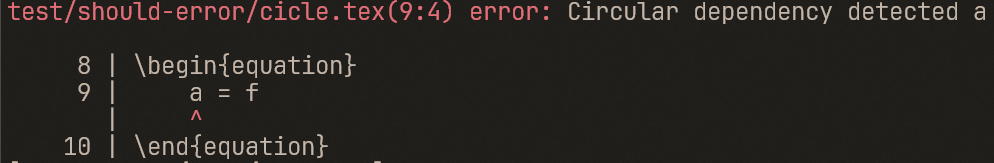
\includegraphics[scale=0.5]{./Imagens/error-circular-deps.png}
    \end{center}
\end{figure}

A resolução de simbolos tem o befenicio de encontrar uma ordem correta de avaliação das declaraçãos, que é crucial para geração de código, já que na linguagem GLSL não é permitido refenciar uma variavel antes dela ser declarada.

A resolução de simbolo considera o escopo do simbolo apropriadamente.

É nessa etapa que detectamos que a função $f$, a BRDF por convenção, existe.


\begin{enumerate}
    \item \textbf{Coleta de Símbolos}:
    \begin{itemize}
        \item Reunir todas as declarações
        \item Registrar símbolos nos escopos apropriados
        \item Inicializar estruturas de rastreamento de dependências
    \end{itemize}

    \item \textbf{Análise de Dependências}:
    \begin{itemize}
        \item Construir o grafo de dependências
        \item Validar referências de símbolos
        \item Estabelecer a ordem de avaliação
    \end{itemize}

    \item \textbf{Validação Final}:
    \begin{itemize}
        \item Verificação de tipos
        \item Verificação do ponto de entrada
        \item Aplicação das regras de escopo
    \end{itemize}
\end{enumerate}



\subsection{Inferencia de Tipos}
Para comentar sobre validdão precisamos informar os tipso que tem XD


A função \verb`infer_type` serve para determinar o tipo de uma expressão sintática (representada por \verb`expr`) em uma árvore abstrata (AST) durante a análise semântica. É usado um conjunto de regras e verificações para inferir e atribuir tipos a expressões com base nas regras matematicas como multiplicação entre numero real e vetor, produtor vetorial dentre dois vetores, assinatura de funções definidas, etc.  Essa função é projetada para lidar com diversas construções que são expressões, como identificadores, operadores prefixados e infixados, chamadas de função e literais.


Inicialmente, a função verifica se o tipo da expressão já foi inferido (\verb`expr.ty_inferred`) e, em caso positivo, retorna o tipo inferido previamente, evitando processamento redundante. Caso contrário, procede com a inferência.

O bloco central da função é um **switch** (parcial) que analisa os diferentes tipos de expressões derivados de \verb`expr`.  
No caso de **identificadores** (\verb`Expr_Identifier`), a função verifica se o identificador representa um vetor especial (\verb`\vec{}`). Por exemplo, podem ser $\omega_i$ que é um vetor ou $\vec{v}$, que pode estar anotado como vector, então seu tipo é inferido como $\mathbb{R^3}$ (Vetor de 3 dimensões). Para identificadores específicos como \verb`Pi` ou \verb`Epsilon`, o tipo é definido como numéro real. Para outros identificadores, a função busca seu tipo no escopo atual, isso é melhor explicado na sessão @@Sessão de funções@@. Se o identificador não for encontrado, dispara um erro, a menos que a opção \verb`allow_invalid` esteja habilitada, permitindo um tipo padrão (\verb`default`).

- Para **operações prefixadas** (\verb`Expr_Prefix`), como raiz quadrada (\verb`Sqrt`) e funções trigonométricas (\verb`Sin`, \verb`Cos`), a função valida que o operando direito seja numérico (\verb`ty_number`), atribuindo o tipo correspondente ao resultado.  
- No caso de **operações infixadas** (\verb`Expr_Infix`), a função realiza a inferência dos tipos dos operandos esquerdo e direito. Se os tipos não forem compatíveis, regras específicas são aplicadas. Por exemplo, a multiplicação ou divisão entre um vetor e um número resulta (ex: $2*\vec{n}$ e $\frac{\vec{u}}{\sqrt{\vec{u} \cdot \vec{u}}}$) no tipo vetor, enquanto operações entre dois vetores ou números seguem regras detalhadas para cada operador.  

---

Outros casos incluem literais, como **números** (\verb`Expr_Number`) e **vetores literais** (\verb`Expr_Vector_Literal`), que têm seus tipos diretamente atribuídos a $\mathbb{R}$ e $\mathbb{R}^3$, respectivamente. Para **chamadas de função** (\verb`Expr_Function_Call`), o tipo da expressão é o tipo do primeiro resultado retornado pela função chamada. A validação dos argumentos passados são feitos em outra função eplicado na sessão @@@

---

A função também realiza validações específicas para evitar inconsistências, como garantir que operações entre vetores sejam semanticamente válidas (e.g., divisão entre vetores não é permitida). Além disso, ao emitir mensagens de erro detalhadas quando confrontada com casos inesperados ou inválidos, erros como os citados da subsessão de error \autoref{@@errors no lexer@@}
---

Em resumo, \verb`infer_type` é uma implementação robusta e flexível de inferência de tipos, essencial para a análise semântica de um compilador. A função assegura que cada expressão receba um tipo coerente com a semântica da linguagem, lidando com uma ampla gama de construções sintáticas e oferecendo suporte extensível para futuras adições à linguagem.


\subsection{Tipos de Expressões}

\subsection{Validação de Funções}
A validação semantica em definições de funções e na chamada de funções é feito com analise similiar. Mas para validar um corretamente, é preciso do conceito de escopo, as variaveis no corpo da função, ou seja o lado direito da equação em uma definição de função, precisa ser manetido na hora de validar se todos os simbolos estão deinifdos.

The function body validation represents the final major phase of function checking. During this phase, the system:
1. Validates all expressions within the function body
2. Infers the return type based on the body's final expression
3. Constructs a complete function type that includes both parameter and return types
4. Ensures all identifier usages within the body conform to their declared types

O processo de validação de uma definição de funçãocomeça com o processamento dos párametros e o managinement do escopo. Quando uma função é definida o s ystema crioa um novo escopo para guardar informaçaões sobre os parametros e a função por sí própria. Isso é cruicial para validar uma chaamda de função e validar as expressões do corpo dessa função. Por exemplo , usando inferencia de tipo para saber s. Cada função recebe um escopo diferente onde o escopo pai é o escopo onde todas as euqações vivem, esse é o escopo global. Isso previne conflito de indetificadores.

Durante a checagem dos paramentros, cada indetificador é feito sua interecia de tipo. Se um parametro for explicitamente marcado com prefixo \verb`\vec`  então ele tera um tipo padrão de $\mathbb{R}^3$, caso contrario é atribuido o tipo de numbero real. 

Seguido do processamento de parametros, o sistema examina todas as expressões do corpo da função, em escial está a validação de identicadores que deve levar em consideração o escopo da função para decidir coisas como, se o identificador está definido se o tipo dele está codizente com o tipo encontrado no escopo. Também considera se está usando algum dos nomes especiais como $\omega_i$, $theta_d$, se não estiver definido nos parametros então dever-se olha no escopo global onde é inserido atuomaticamente esses identificadres especiais e seus tipos. Por exemplo, se o parametro $\vec{x}$ é declarado como vetor, todos o uso de indetificado 'x' dentro do corpo da funlão deve manter as caracteristicas de operação de vetor, caso contrario um erro é reportado.

Algo muito similiar acontece na chamada de funções, todos os argumetnos passados para essa função, feito sua inferencia de tipo e checkado se corresponde à assinatura de da função que está sendo chamda, o \verb`Type_Funcion`.
Por exemplo considere as equações no \autoref{cod-type-mismatch}, $g$ possui o tipo $\mathbb{R}\mathbb{R} \to \mathbb{R}$. O valor da expressão de chamada de função inteiro tem o tipo do contradominio de C, nesse caso o contra dominio corresponde ao valor possivel para f, que pode ser um numero para ou um vector de 3 dimensoes que representa cor, mas o segundo argumento passado mara g no RHS de f, está incorreto, pois passamos um vetor quando se espera um numero real, e portando temos o erro ilustrado na \autoref{fig-type-mismatch}, que diz que extamente o segundo argumento está incorreto.
\begin{codigo}[htb]
    \caption{\small Equação com uso incorreto de tipos na chamada de função. }
    \label{cod-type-mismatch}
\begin{lstlisting}[language=tex, numbers=none, frame=none, inputencoding=latin1]
\begin{equation}
    g(a, x) = a*x*x
\end{equation}

\begin{equation}
    f = g(1, \vec{1,1,1})
\end{equation}

\end{lstlisting}
\end{codigo}

\begin{figure}[H]
    \caption{\label{fig-type-mismatch} \small Erro gerado por uso incorreto de tipos na chamada de função.}
    \begin{center}
        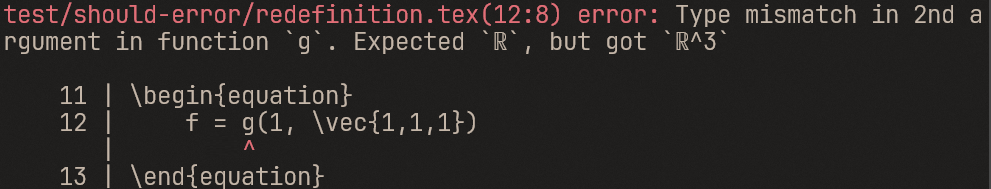
\includegraphics[scale=0.5]{./Imagens/error-type-mismatch.png}
    \end{center}
\end{figure}

Scope-based validation manages symbol visibility and access, ensuring that variables are only accessed within their proper scope and that shadowing follows language rules.

\subsection{Validação de Equaçoes}
Declarações passam por um processo rigososo de validão

Para todos os identificadore, é cirado um escopo global contendo todas os identificadres. Isso mantém visibilidade do simbolo  previne conflito de nomes. Declarações de equação passa pela validação de os lado esquerdo das equações (lhs) e garante que está definido, isso é feito depois da etapa de colega e ordenação \autoref{colega e ordenação de equações}. Cada LHS deve ser out um identificador valido ou a definiç~eos de uma função. Esse processro também checka por redefinição de symbolos, para prefinir multiplas declarações do mesmo simbolo no mesmo escopo.


Todas as violações semanticas como mismatch de tipos ou usar valor escalar quando um vetor é esperado é reportado para o usuáriojustamente com informações sobre o contexto e o local de erro.


Essta etapa de validação semantica provê toda a ffoundatioon para ter um programa correto gerado, explicitamente importante para a próxima estapa, que é a geração de código.
A função \verb`check_expr` verifica a semântica e os tipos de uma expressão representada em uma AST (Abstract Syntax Tree). Ela opera em diferentes tipos de expressão (identificadores, chamadas de função, operadores, etc.), garantindo que elas sigam as regras do sistema de tipos e da linguagem.

A todo momento os identificadores embutidos estabelicidos na conveções desse trabalho são adicionado a tabela de simbolos, definidos e pronto para uso. \autoref{cod-builtins}

\begin{codigo}[htb]
    \caption{\small Identificadores embutidos pela convenção deste trabalho. }
    \label{cod-builtins}
\begin{lstlisting}[language=C, numbers=none, frame=none, inputencoding=latin1]
BUILTIN_IDENTIFIERS :: []string {
    `\max`,
    `\pi`,
    `\epsilon`,
    `\theta{h}`,
    `\vec{n}`,
    `\vec{h}`,
    `\vec{\omega{i}}`,
    `\theta{i}`,
    `\phi{i}`,
    `\vec{\omega{o}}`,
    `\theta{o}`,
    `\phi{o}`,
    `\theta{h}`,
    `\theta{d}`,
}
\end{lstlisting}
\end{codigo}


\subsubsection{Casos mais relevantes}

@Adicione o caso binário@
\begin{itemize}
    
    \item Identificadores (\verb`Expr_Identifier`): 
      Verifica se o identificador está definido no escopo atual. Caso contrário, gera um erro com a mensagem apropriada. Se estiver definido:
    \item **Chamadas de Função (\verb`Expr_Function_Call`)**:  
      A função realiza várias validações:
      - Verifica se a expressão da esquerda é um identificador válido.
      - Confirma que o identificador refere-se a um símbolo do tipo função.
      - Garante que o número e os tipos dos argumentos correspondem aos parâmetros esperados.
      - Para cada argumento, chama recursivamente \verb`check_expr`.
    \item **Expressões com Prefixo (\verb`Expr_Prefix`)**:  
      Avalia operadores como \verb`-`, \verb`+`, ou funções como `sqrt()` e `sin()`. Por exemplo:
      - Em \verb`sqrt(x)`, verifica se `x` é um número (\verb`ty_number`). Caso contrário, exibe um erro.
      - Para operadores básicos como \verb`-` e `+`, a inferência de tipo já determina o comportamento correto.
    \item **Literais de Vetor (\verb`Expr_Vector_Literal`)**:  
      Verifica se o vetor tem exatamente 3 dimensões. Caso contrário, gera um erro indicando o formato esperado.
\end{itemize}






\begin{codigo}[htb]
    \caption{\small Validação de parametros de uma função. }
    \label{cod-parametros-validation}
\begin{lstlisting}[language=C, numbers=none, frame=none, inputencoding=latin1]
// ...
parameter_types := [dynamic]^Type{}
scope_enter(fn_sym.scope) {
    for &parameter in fn.parameters {
        parameter_key := key_from_identifier(parameter)
        ty := infer_type(parameter, true, ty_number)
        parameter_sym.type = ty
        append(&parameter_types, ty)
    }
}
// ...
\end{lstlisting}
\end{codigo}


\begin{codigo}[htb]
    \caption{\small Validação de um uníco identificador. }
    \label{cod-check-single-ident}
\begin{lstlisting}[language=C, numbers=none, frame=none, inputencoding=latin1]

check_single_identifier :: proc(parameters: []^ast.Expr_Identifier, ident: ^ast.Expr_Identifier) {
    infer_type(ident)
    ident_key := key_from_identifier(ident)
    // Validates type consistency between declaration and usage
    if !is_type_equal(ident.ty_inferred, p.ty_inferred) {
        error(ident.identifier, "Parameter `%v` being use as type `%v` when the expected type is `%v`", ...)
    }
}
\end{lstlisting}
\end{codigo}


\section{Validação de Definição e Declaração de Função na Análise Semântica}

\subsection{Validação da Definição de Função}
O procedimento \verb`check_function_definition` implementa um sistema de validação abrangente para definições de função, garantindo segurança de tipos e consistência de parâmetros.

\subsubsection{Fase 1: Processamento de Parâmetros}
Aspectos principais:
\begin{itemize}
    \item Cria um novo escopo para os parâmetros da função
    \item Inferência de tipos para cada parâmetro
    \item Mantém informações sobre o tipo dos parâmetros
    \item Tratamento de tipo padrão (número se não for vetor)
\end{itemize}

\subsubsection{Fase 2: Validação de Identificadores}
Assim como no parser, temos uma correspondência entre os tipos da árvore sintática com \verb|Expr_Identifier|, \verb|Expr_Infix|, etc., com funções que podem ser indiretamente recursivas, como \verb|check_single_identifier| (\autoref{cod-check-single-ident}), \verb|check_expr|, etc.

\subsubsection{Fase 3: Validação do Corpo da Função}
\begin{codigo}[htb]
    \caption{\small Validação do corpo da função.}
    \label{cod-function-body-validation}
\begin{lstlisting}[language=C, numbers=none, frame=none, inputencoding=latin1]
scope_enter(fn_sym.scope) {
    check_expr(body)
    body_type := infer_type(body)
    result_types := [dynamic]^Type{body_type}
    fn_type := make_function_type(parameter_types[:], result_types[:])
}
\end{lstlisting}
\end{codigo}

Passos principais:
\begin{itemize}
    \item Validação de expressões
    \item Inferência do tipo de retorno
    \item Construção do tipo de função
    \item Gerenciamento de escopo
\end{itemize}

\subsection{Tratamento de Declaração de Equação}
\begin{codigo}[htb]
    \caption{\small Tratamento de declaração de equação.}
    \label{cod-equation-declaration}
\begin{lstlisting}[language=C, numbers=none, frame=none, inputencoding=latin1]
case ^Decl_Equation:
    check_decl(s)
\end{lstlisting}
\end{codigo}

\subsection{Mecanismos de Segurança de Tipos}
A implementação garante segurança de tipos através de vários mecanismos:

\begin{itemize}
    \item \textbf{Validação de Tipo de Parâmetro}
    \begin{itemize}
        \item Verificação explícita de tipos para parâmetros
        \item Tratamento de tipo vetor (reconhecimento do prefixo \verb|\vec|)
        \item Atribuição de tipo padrão
    \end{itemize}

    \item \textbf{Validação Baseada em Escopo}
    \begin{itemize}
        \item Gerenciamento hierárquico de escopo
        \item Controle de visibilidade de símbolos
        \item Isolamento de escopo de parâmetros
    \end{itemize}

    \item \textbf{Detecção de Erros}
    \begin{itemize}
        \item Detecção de incompatibilidade de tipos
        \item Validação de uso de parâmetros
        \item Verificação de violação de escopo
    \end{itemize}
\end{itemize}

\subsection{Detalhes Técnicos da Implementação}

\subsubsection{Resolução de Símbolos}
\begin{itemize}
    \item Símbolos de parâmetros são resolvidos dentro do escopo da função
    \item Inferência de tipos é realizada para todos os identificadores
    \item Consistência de tipos é aplicada em todo o corpo da função
\end{itemize}

\subsubsection{Gerenciamento de Escopo}
\begin{codigo}[htb]
    \caption{\small Gerenciamento de escopo na validação do corpo da função.}
    \label{cod-scope-management}
\begin{lstlisting}[language=C, numbers=none, frame=none, inputencoding=latin1]
scope_enter(fn_sym.scope) {
    // Validação do corpo da função
    check_expr(body)
    // Inferência e validação de tipo
    body_type := infer_type(body)
}
\end{lstlisting}
\end{codigo}
\section*{Validação de Campo de Declaração e Definição de Funções na Análise Semântica}

Este documento descreve o funcionamento das funções \texttt{check\_field} e \texttt{check\_function\_definition}, incluindo a validação semântica de campos, declaração de equações e definições de funções. 

\subsection*{Fluxo Geral da Função \texttt{check\_field}}

A função \texttt{check\_field} garante que os campos de uma estrutura ou declaração estejam semanticamente corretos. Esse processo segue as etapas abaixo:

\begin{itemize}
  \item \textbf{Validação do LHS (Chave):}  
  O lado esquerdo deve ser um identificador ou definição de função. Erros de validação são detalhados com mensagens explicativas.

  \item \textbf{Definições de Função:}  
  Chaves que representam definições de função são delegadas à função \texttt{check\_function\_definition}, que valida os parâmetros e o corpo da função.

  \item \textbf{Validação do RHS (Valor):}  
  O valor (\texttt{field.value}) é verificado recursivamente com \texttt{check\_expr}. Caso o tipo não esteja inferido, a inferência é realizada.

  \item \textbf{Comparação de Tipos:}  
  Após a inferência, verifica se os tipos do LHS e RHS são compatíveis. Inconsistências são detalhadas nas mensagens de erro.

  \item \textbf{Gerenciamento de Símbolos:}  
  Os símbolos representam variáveis ou funções na linguagem. Caso o símbolo já exista, ele é atualizado; caso contrário, um novo símbolo é criado.
\end{itemize}

\subsection*{Validação de Definições de Funções}

A função \texttt{check\_function\_definition} é responsável pela validação completa de definições de funções. Ela assegura a consistência dos parâmetros e a segurança de tipos.

\subsubsection*{Fase 1: Processamento de Parâmetros}
\begin{itemize}
  \item Cria um novo escopo para os parâmetros da função.
  \item Realiza inferência de tipos para cada parâmetro.
  \item Lida com tipos padrão (e.g., vetor para prefixos \textbackslash{}vec).
\end{itemize}

\subsubsection*{Fase 2: Validação do Identificador}
Correspondências entre a árvore sintática e os tipos são validadas recursivamente por funções como \texttt{check\_single\_identifier} e \texttt{check\_expr}.

\subsubsection*{Fase 3: Validação do Corpo da Função}
O corpo da função é validado em um escopo isolado:
\begin{itemize}
  \item Expressões são verificadas com \texttt{check\_expr}.
  \item O tipo de retorno é inferido e comparado com o tipo declarado.
  \item O tipo da função é construído com base nos parâmetros e resultados.
\end{itemize}

\begin{codigo}[htb]
    \caption{\small Estruturas que representam o tipo de um expressão da AST.}
    \label{cod-types-structs}
\begin{lstlisting}[language=C, numbers=none, frame=none, inputencoding=utf8]
case ^Decl_Equation:
    check_decl(s)

scope_enter(fn_sym.scope) {
    // Validação do corpo da função
    check_expr(body)
    // Inferência e validação de tipo
    body_type := infer_type(body)
    result_types := [dynamic]^Type{body_type}
    fn_type := make_function_type(parameter_types[:], result_types[:])
}
\end{lstlisting}
\end{codigo}

\subsection*{Mecanismos de Segurança de Tipos}

A implementação garante a segurança de tipos por meio de:
\begin{itemize}
  \item \textbf{Validação de Parâmetros:}  
  Checagem explícita de tipos para parâmetros e reconhecimento de vetores (\textbackslash{}vec).

  \item \textbf{Gerenciamento de Escopos:}  
  Uso de operações hierárquicas (\texttt{scope\_enter}/\texttt{scope\_exit}) para evitar conflitos de símbolos.

  \item \textbf{Detecção de Erros:}  
  Identificação de inconsistências de tipo, violações de escopo e uso inválido de parâmetros.
\end{itemize}

\subsection*{Exemplo de Declaração de Equação}

A seguir, apresentamos um trecho que demonstra o manuseio de uma declaração de equação:
\begin{codigo}[htb]
    \caption{\small Declaração de Equação na Análise Semântica.}
    \label{cod-equation-decl}
\begin{lstlisting}[language=C, numbers=none, frame=none, inputencoding=utf8]
case ^Decl_Equation:
    if scope.has_symbol(lhs.name):
        raise_error("Redeclaração de símbolo:", lhs.name)
    else:
        symbol_table.add(lhs.name, lhs.type)
    check_expr(rhs)
\end{lstlisting}
\end{codigo}


%     \
% A função `check_field` garante que um campo de uma estrutura ou declaração (LHS = chave, RHS = valor) esteja semanticamente correto. Esse processo inclui a validação de tipos, verificações de escopo e atualizações nos símbolos associados.
%
% #### **Fluxo Geral**
%
% 1. **Validação do LHS (Chave):**
%    - O lado esquerdo deve ser um identificador ou definição de função.  
%    - Se o LHS for inválido, um erro é exibido com detalhes do problema.
%
% 2. **Definições de Função:**  
%    Se a chave for uma definição de função, o sistema delega o processamento para `check_function_definition`, que cuida de verificar parâmetros, tipos de retorno e o corpo da função.
%
% 3. **Validação do RHS (Valor):**
%    - Verifica recursivamente o lado direito (`field.value`) chamando `check_expr`.
%    - Caso o tipo não esteja inferido, realiza a inferência para garantir que o valor esteja bem definido.
%
% 4. **Comparação de Tipos:**
%    - Após inferir ambos os tipos (LHS e RHS), verifica se eles coincidem.
%    - Erros de incompatibilidade são detalhados, apontando o tipo esperado e o tipo real.
%
% 5. **Gerenciamento de Símbolos:**  
%    Os símbolos representam variáveis ou funções na linguagem.  
%    - Se o símbolo já existe no escopo, atualiza suas informações (tipo, valor, etc.).
%    - Caso contrário, cria um novo símbolo e o adiciona ao escopo.
%
% ---
%
% ### **Pontos-chave de ambas as funções**
%
% - **Recursividade:**  
%   Ambas as funções lidam com estruturas aninhadas chamando recursivamente `check_expr`. Isso permite a validação de expressões complexas, como chamadas de funções aninhadas ou operadores compostos.
%
% - **Separação entre Inferência e Checagem:**  
%   A separação entre inferência de tipos (`infer_type`) e verificação de tipos (`check_expr`) torna o design mais modular, ainda que cause alguma sobreposição.
%
% - **Mensagens de Erro Detalhadas:**  
%   As mensagens fornecem contexto suficiente para o desenvolvedor corrigir o problema, indicando onde ocorreu o erro e qual foi o tipo esperado/recebido.
%
% - **Gerenciamento de Escopos:**  
%   Operações como `scope_enter` e `scope_exit` permitem que blocos de código ou funções sejam avaliados em contextos locais, evitando conflitos de símbolos globais.
%
% Essas características fazem com que ambas as funções sejam peças fundamentais para a validação semântica e a segurança de tipos no compilador.
%
%
% -----------
% Também deve considerar colisão de equações já definidas, por exemplo f = 2 e depois f=3, detectamops um problema, dentro de uma definição de função, pode-se usart qualquer simbolo definido em uma equação anterior, ou seus parametros, para declarar que a variable dessa função é um vetor, basta prefixar com $\vec$
%
%
% ---
% # Function Definition and Declaration Validation in Semantic Analysis
%
% ## Function Definition Validation
% The \verb`check_function_definition` procedure implements a comprehensive validation system for function definitions, ensuring type safety and parameter consistency.
%
% ### Phase 1: Parameter Processing
% Key aspects:
% 1. Creates new scope for function parameters
% 2. Infers types for each parameter
% 3. Maintains parameter type information
% 4. Default type handling (number if not vector)
%
% ### Phase 2: Identifier Validation
% Assim como no parser temos uma uma correspondencia entre os tipos da arvore sintatica com Expr_Identifier, Expr_Infix, etc.. com fnção que podem ser indiretamente recursivas como \verb"check_single_identifier" (\autoref{cod-check-single-ident}), \verb"check_expr", etc...
% ### Phase 3: Function Body Validation
% scope_enter(fn_sym.scope) {
%     check_expr(body)
%     body_type := infer_type(body)
%     result_types := [dynamic]^Type{body_type}
%     fn_type := make_function_type(parameter_types[:], result_types[:])
% }
%
% Key steps:
% 1. Expression validation
% 2. Return type inference
% 3. Function type construction
% 4. Scope management
%
%
% Features:
% 1. New scope creation for blocks
% 2. Recursive statement validation
% 3. Proper scope cleanup
%
% ### Equation Declaration Handling
% ```odin
% case ^Decl_Equation:
%     check_decl(s)
% ```
%
% ## Type Safety Mechanisms
%
% The implementation ensures type safety through several mechanisms:
%
% 1. **Parameter Type Validation**
%    - Explicit type checking for parameters
%    - Vector type handling (`\vec` prefix recognition)
%    - Default type assignment
%
% 2. **Scope-Based Validation**
%    - Hierarchical scope management
%    - Symbol visibility control
%    - Parameter scope isolation
%
% 3. **Error Detection**
%    - Type mismatch detection
%    - Parameter usage validation
%    - Scope violation checking
%
% ## Technical Implementation Details
%
% ### Symbol Resolution
% 1. Parameter symbols are resolved within function scope
% 2. Type inference is performed for all identifiers
% 3. Type consistency is enforced throughout the function body
%
% ### Scope Management
% ```odin
% scope_enter(fn_sym.scope) {
%     // Function body validation
%     check_expr(body)
%     // Type inference and validation
%     body_type := infer_type(body)
% }
% ```
%
% ### Error Handling
% The system provides detailed error messages for:
% 1. Type mismatches
% 2. Invalid parameter usage
% 3. Scope violations
% 4. Vector notation issues

